\documentclass{patmorin}
\usepackage{pat,graphicx,amsmath}
\usepackage[mathlines]{lineno}
\linenumbers
\listfiles


\newcommand{\eps}{\epsilon}
\newcommand{\depth}{\mathrm{depth}}
%\usepackage{wasysym}
%\newcommand{\poly}{\hexagon}
\newcommand{\poly}{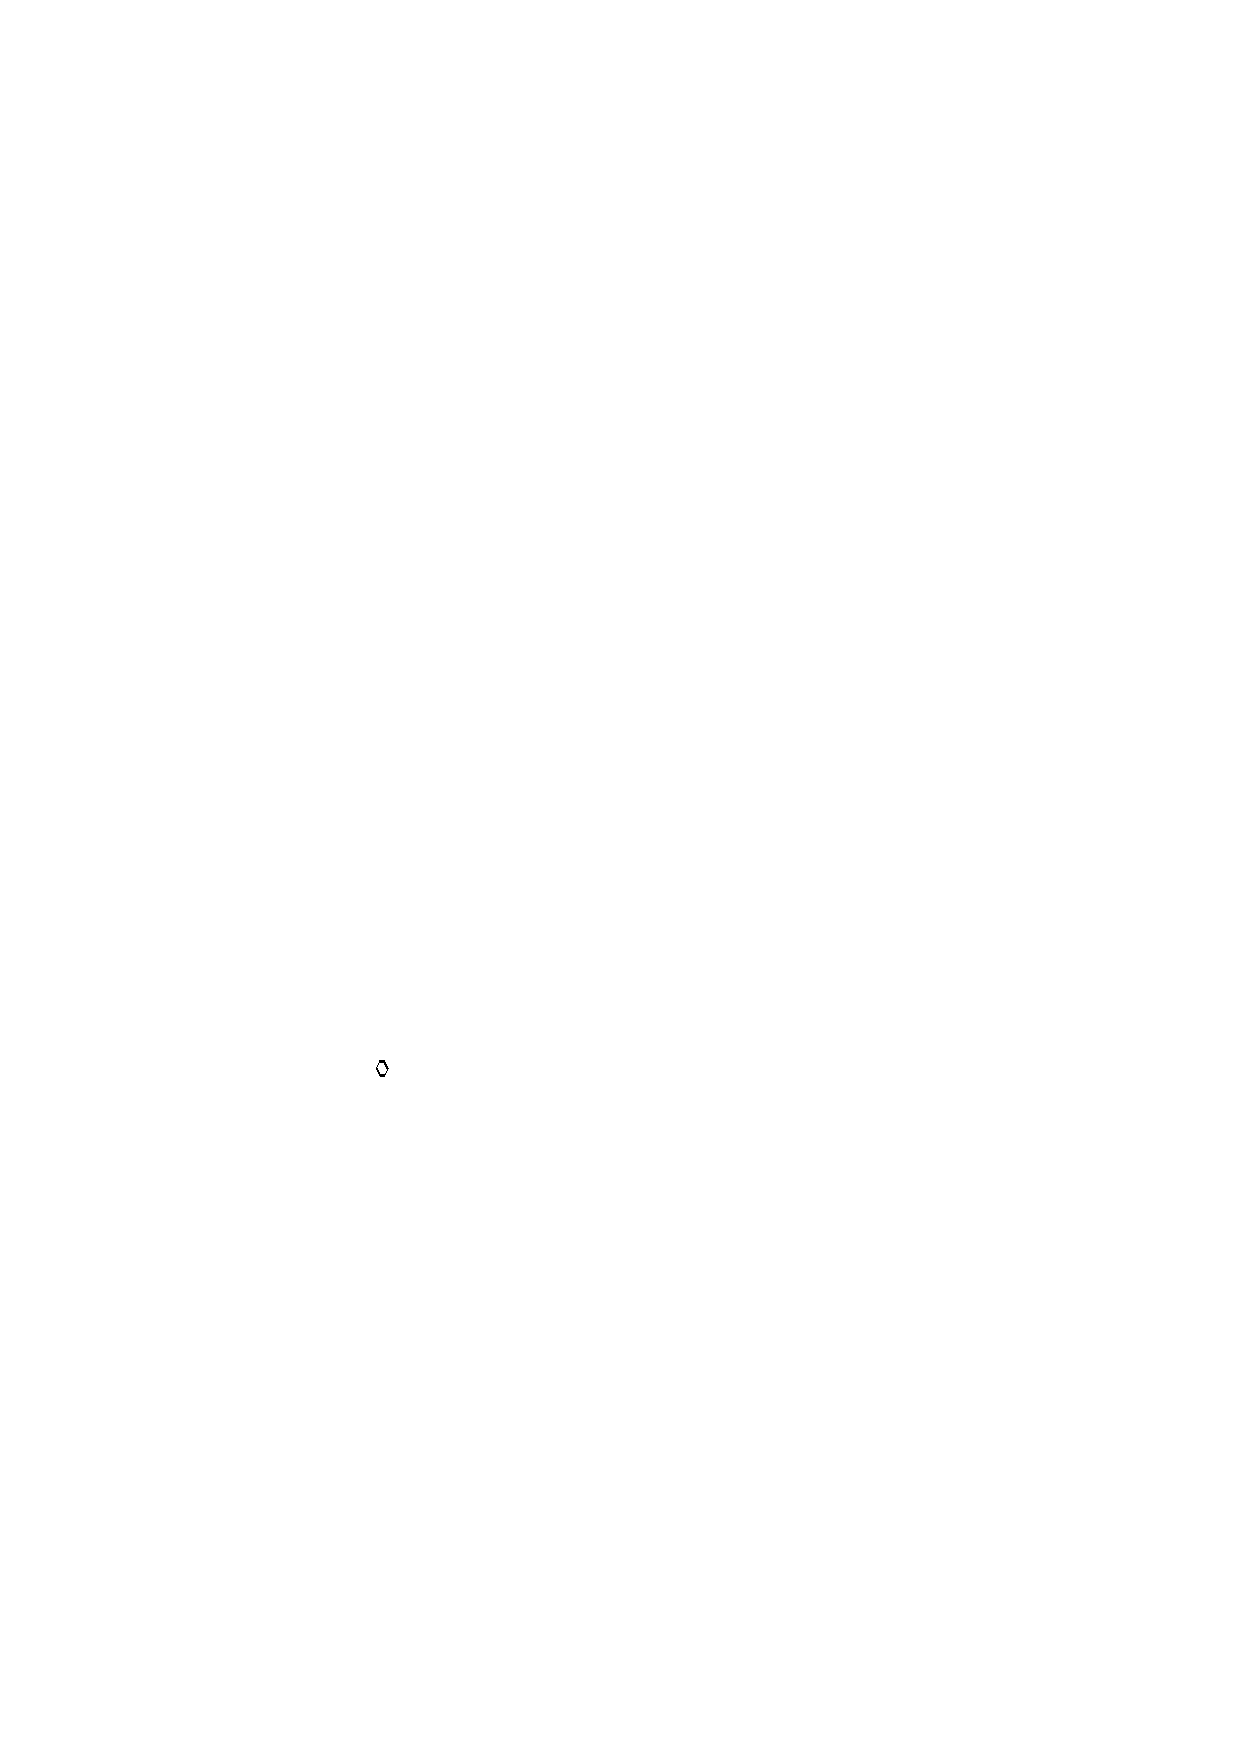
\includegraphics{poly}}
% consider also \pentagon \varhexagon \hexagon with package wasysym

\title{\MakeUppercase{Working Title: Distribution-Sensitive Everything}}

\author{Prosenjit~Bose, 
        Luc~Devroye,
	Karim~Dou\"{\i}eb, 
	Vida~Dujmovi\'c, 
	James~King, and 
	Pat~Morin}

\begin{document}
\maketitle

\begin{abstract}
Let $\mathcal{P}:\R^d\rightarrow A$ be a query problem over
$\R^d$ for which there exists a data structure $\mathcal{S}$ that can
compute $P(q)$ in $O(\log n)$ time for any query point $q$.  Let $D$ be a
probability measure over $\R^d$ representing a distribution of queries.
We describe a data structure $T=T(\mathcal{P},D)$ of size $O(n^\eps)$
that can be used as a filter that quickly computes $\mathcal{P}(q)$
for some query values in $\R^d$ and relies on $\mathcal{S}$ for the
remaining queries.  With this filter, the expected query time for a point
drawn according to $D$ is $O(1+ H^*)$, where $H^*$ is a lower-bound on
the expected cost of any linear decision tree that solves $\mathcal{P}$.

This result has a number of applications, including distribution-sensitive
data structures for point location in 2-d, point-in-polytope testing in
3-d, nearest-neighbour queries in $\R^d$, point-location in arrangements
of hyperplanes in $\R^d$, and many other geometric searching problems
that can be solved in the linear-decision tree model.
\end{abstract}

\section{Introduction}

Let $\mathcal{P}:\R^d\rightarrow A$ be a query problem over $\R^d$.
That is, $\mathcal{P}$ represents a searching problem in which every query
$p\in\R^d$ has an answer the set $A$ of possible answers.  Suppose,
further that there exists a data structure $\mathcal{S}$ that can
compute $P(q)$ in $O(\log n)$ time for any query point $q$. Let $D$ be a
probability measure over $\R^d$ representing a distribution of queries.
We describe a data structure $T_{\mathcal{P},D}$ of size $O(n^{\eps})$
that can be used as a filter that quickly computes $\mathcal{P}(q)$
for some query values in $\R^d$ and relies on $\mathcal{S}$ for the
remaining queries.  With this filter, the expected query time for a point
drawn according to $D$ is $O(1+ H^*)$, where $H^*$ is a lower-bound on
the expected cost of any linear decision tree that solves $\mathcal{P}$
when queries are drawn according to $D$.

The remainder of this paper is organized as follows: \Secref{prelim}
presents some preliminary definitions and results. \Secref{filter}
presents the data structure and algorithms for constructing it.
\Secref{lower-bound} proves that this data structure matches the query
time of any linear decision tree.  \Secref{applications} presents
some of the geometric applications of this data structure. Finally,
\secref{conclusions} summarizes and concludes with open problems.

\section{Preliminaries}
\seclabel{prelim}

Throughout this paper, the underlying dimension $d$ is a constant, and
other constants defined throughout the paper may (implicitly) depend
on $d$.  A \emph{simplex} in $\R^d$ is the common intersection of a
set of at most $d+1$ closed halfspaces in $\R^d$. Note that, under this
definition, simplices need not be bounded and $\R^d$ as well as $\emptyset$ are both simplices.

Throughout this paper, we assume an underlying probability measure
$D$ over $\R^d$.  All expectations and probabilities are (implicitly)
with respect to $D$.  For any subset $X\subseteq\R^d$, $\Pr(X)$ refers
to $D(X)$.  We use the notation $D_{|X}$ to denote the distribution $D$
conditioned on $X$, i.e., $D_{|X}(Y)=\Pr(Y\mid X)=\Pr(X\cap Y)/\Pr(X)$
for all $Y\subseteq\R^d$.  If $F=\{X_1,\ldots,X_k\}$ are non-overlapping
subsets of $\R^d$ then the \emph{entropy} of $F$, denoted $H(F)$ is
\[
    H(F) = \sum_{i=1}^k \Pr(X_i|\cup F)\log(1/\Pr(X_i|\cup F)) \enspace .
\]
The probability measure $D$ is used as an input to our algorithms.
We assume that the algorithm has access to $D$ through two oracles.
The \emph{Measure Oracle} allows, for any simplex $\Delta$, to determine
$\Pr(\Delta)$ in constant time.  The \emph{Sampling Oracle} allows us
to draw a random sample $p$ from the distribution $D$.

A \emph{query problem} over $\R^d$ is a function
$\mathcal{P}:\R^d\rightarrow A$ where $A$ is some set of \emph{answers}.
We assume the existence of two oracles that allow access to $\mathcal{P}$.
The \emph{Backup Oracle} allows us to compute $\mathcal{P}(p)$ for
any query point $p$, but requires $O(\log n)$ time to do so.  The
\emph{Interference Oracle} allows us to test, for any simplex $\Delta$,
if $\mathcal{P}(p)=\mathcal{P}(q)$ for every pair $p,q\in\Delta$.
The running time of the Interference Oracle will be unspecified.
When discussing applications in \secref{applications}, implementations
of the Interference Oracle for particular problems will be described.

A \emph{linear decision tree} for $\mathcal{P}$ is a rooted ordered
binary tree in which each internal node $v$ is labelled with a linear
inequality $a_{v,1}x_1 + a_{v,2}x_2 + \cdots a_{v,d}x_d + a_{v,d+1} > 0$,
and each leaf $w$ is labelled with an element $w_A\in A$.  A query point
$p=(x_1,\ldots,x_d)$ follows a root-to-leaf path, proceeding to the right
child of $v$ if it satisfies the inequality and the left child of $v$
if it does not.  For a linear decision tree $T$ and a point $p\in\R^d$,
we denote by $T(p)$ the label of the leaf on the root-to-leaf path
for $p$ in $T$.  A linear decision tree \emph{solves} $\mathcal{P}$ if
$T(p)=\mathcal{P}(p)$ for all $p\in\R^d$. The \emph{depth} of a node $v$
in a rooted tree $T$, denoted $\depth_T(v)$, is the number of edges on
the path from $v$ to the root of $T$.  The \emph{(expected) cost} of a
linear decision tree, denoted $\mu_D(T)$, is the expected depth of the
leaf reached when $p$ is drawn according to the probability measure $D$.


\section{The Data Structure}
\seclabel{data-structure}

In this section we describe a data structure $T_{\mathcal{P},D}$ called
the \emph{filter tree} that, in conjunction with a Backup Oracle, yields
a data structure for $\mathcal{P}$ that has expected query time that
is within a constant factor of the expected query time of any linear
decision tree $T^*$ for $\mathcal{P}$.  The filter tree is based on
simplicial partitions, from the field of geometric range searching:

\begin{thm}[Matou\v{s}ek 1992]\thmlabel{point-partition}
There exists a constant $c$ such that, for any set $S$ of $m$
points in $\R^d$ and any constant $r$, there exists a sequence
$\langle \Delta_1,\ldots,\Delta_r\rangle$ of closed simplices such that
  \begin{enumerate}
    \item $\bigcup_{i=1}^r \Delta_i = \R^d$,
    \item $\left|\Delta_i \cap S\setminus
    \left(\bigcup_{j=1}^{i-1}\Delta_j\right)\right| \le 2m/r$, and
    \item For any hyperplane $\ell$, there are at most $cr^{1-1/d}$ elements of
  $\{\Delta_1,\ldots,\Delta_r\}$ whose interiors intersect $\ell$.
  \end{enumerate}
  The sequence of simplices $\Delta_1,\ldots,\Delta_r$ can be computed
  in $O(m)$ time.
\end{thm}

Note that Part~2 of \thmref{point-partition} is not in the original
statement of the theorem, but follows from Matou\v{s}ek's incremental
construction of $\Delta_1,\ldots,\Delta_r$ \cite{m92}.

%We require a slightly more restricted version of this Theorem in which
%the $\Delta_i$ are restricted to lie some containing simplex $\Delta$:
%
%\begin{cor}\corlabel{point-partition}
%There exists a constant $c$ such that, for any set $S$ of $m$ points
%contained in some simplex $\Delta \subseteq \R^d$ and any constant $r<m$,
%there exists a sequence
%$\langle \Delta_1,\ldots,\Delta_{r}\rangle$ of closed simplices such that
%  \begin{enumerate}
%    \item $\bigcup_{i=1}^{r} \Delta_i = \Delta$,
%    \item $\left|\Delta_i \cap S\setminus
%    \left(\bigcup_{j=1}^{i-1}\Delta_j\right)\right| \le 2m/r$, and
%    \item For any hyperplane $\ell$, there are at most $cr^{1-1/d}$ elements of
%  $\{\Delta_1,\ldots,\Delta_{r}\}$ whose interiors intersect $\ell$.
%  \end{enumerate}
%  The sequence of simplices $\Delta_1,\ldots,\Delta_{r}$ has $r=O(r)$
%  elements and can be computed in $O(m)$ time.
%\end{cor}
%
%\begin{proof}
%The theorem is obtained by applying \thmref{point-partition} and then
%further subdividing the resulting sequence $\Delta_1,\ldots,\Delta_r$
%of simplices.  For each $\Delta_i$, we compute the common
%intersection $P_i=\Delta_i \cap \Delta$. The resulting polytope $P_i$
%is the common intersection of at most $2d$ halfspaces and, by the
%Upper Bound Theorem \cite{m70}, has $O(d^{\floor{d/2}})$ vertices
%and can therefore be partitioned into $O(d^{\floor{d/2}})$ simplices
%$\Delta_{i,1},\ldots,\Delta_{i,r_i}$ using the bottom-vertex triangulation
%\cite{c88}.
%
%The resulting sequence of $r=O(r)$ simplices certainly has properties 1
%and 2 of the theorem.  The sequence also has property 3, though the
%constant $c$ is multiplied by a factor of $O(d^{\floor{d/2}})=O(1)$.
%\end{proof}

Let $\Delta_i^*$ denote the incremental difference
$\Delta_i^*=\Delta_i\setminus\bigcup_{j=1}^{i-1}\Delta_j$.  Let $S$
be a set of $m$ points in $\R^d$. Then the \emph{partition tree}
$T_S$ for $S$ is a rooted ordered tree obtained by recursively
applying \thmref{point-partition}.  The root of $T_S$ has $r$ children
corresponding to the simplices $\Delta_1,\ldots,\Delta_{r}$ obtained
by applying \thmref{point-partition} to $S$.  The $i$th child of the
root is itself the root of the partition tree $T_{S\cap\Delta_i^*}$
for $S\cap\Delta_i^*$. This recursive process stops when a node is
empty of points in $S$ or its depth exceeds $\floor{\eps\log_r m}$,
for some constant parameter $\epsilon\in(0,1]$.

Next we define some regions, $\Delta(v)$, $\poly(v)$, and $\Xi(v)$,
that are associated with each node $v$ of $T_S$.  Every node $v$ in
$T_S$, except the root of $T_S$, is naturally associated with a simplex
$\Delta(v)$ that was obtained from \thmref{point-partition} and that
generated $v$.  For the root of $T_S$, we define $\Delta(v)=\R^d$.

For a node $v$ of $T$ whose ancestors are $v=v_0, v_1,\ldots,v_i$
we define $\poly(v)=\bigcap_{j=0}^i \Delta(v_i)$.  Note that
$\poly(v)\subseteq\Delta(v)$, and that $\poly(v)$ is a convex polytope
that has $O(((d+1)(i+1))^{\floor{d/2}})=O(i^{\floor{d/2}})$ vertices since
it is the intersection of at most $(d+1)(i+1)$ halfspaces \cite{m70}.

For a point $p\in\R^d$, the \emph{search path} for $p$ in $T_S$ starts
at the root and proceeds to the first child $i$ such $p\in\Delta_i$
(note that this implies $p\in\Delta_i^*$) and this process is applied
recursively until reaching a leaf of $T_S$.  In this way, for every $v$
of the partition tree there is a maximal subset $\Xi(v)\subseteq \R^d$
such that the search path for every point in $p\in\Xi(v)$ contains $v$.
Note that $\Xi(v)\subseteq \poly(v)\subseteq \Delta(v)$, but that
$\Xi(v)$ is not necessarily convex or even connected.

The following theorem summarizes the properties of the partition tree
$T_{S}$ \cite{m92} (each property is inherited from the corresponding
property of the simplicial partition in
\thmref{point-partition}):

\begin{thm}\thmlabel{point-partition-tree}
Let $S$ be a set of $m$ points in $\R^2$, let $T_S$ denote the partition
tree described above, and let $V_i$ denote the set of $r^i$ nodes of
$T_S$ at depth $i$.  There exists a constant $c$, independent of $r$,
such that the partition tree $T_S$ has the following properties, for
every $i\in\{0,\ldots,\lfloor\eps\log_r n\rfloor\}$:
\begin{enumerate}
  \item $\{\Xi(v) : v\in V_i\}$ is a partition of $\R^2$,  
  \item For every node $v\in V_i$, $|S\cap\Xi(v)| \le m(2/r)^i$, and 
  \item For any hyperplane $\ell$, the number of nodes in $V_i$ such that
        $\ell$ intersects the interior of $\poly(v)$ is at most
        $(cr^{1-1/d})^i$.
  \end{enumerate}
  The partition tree $T_S$ can be constructed from $S$ in $O(m\log m)$ time.
\end{thm}

%\noindent\textbf{Remark:} The use of \thmref{point-partition} (as
%opposed to \thmref{point-partition}) is crucial for the construction
%of $T_{S,\R^2}$ since, otherwise, the resulting tree will not have
%Property 3.

Restating \thmref{point-partition} in terms of probability distributions,
we have:

\begin{thm}\thmlabel{prob-partition-tree} 
  Let $S$ be a sample of $m$ points in $\R^d$ drawn i.i.d.\ according
  to probability measure $D$, let $T_D=T_S$ denote the partition tree
  given by \thmref{point-partition-tree}, and let $V_i$ denote the set
  of $r^i$ nodes of $T_D$ at depth $i$.  There exists a constant $c$,
  independent of $r$, $m$ and $D$, such that with probability at least
  $1-O(m^{-\gamma})$, $T_D$ has the following properties, for every
  $i\in\{0,\ldots,\lfloor\alpha\log_r n\rfloor\}$:
  \begin{enumerate}
    \item $\{\Xi(v) : v\in V_i\}$ is a partition of $\R^2$,  
    \item For every node $v\in V_i$, $\Pr(\Xi(v)) \le
           (3/r)^i+O(m^{-\delta})$, and
    \item For any hyperplane $\ell$, the number of nodes in $V_i$
         such that $\ell$ intersects the interior of $\poly(v)$ is at
         most $(cr^{1-1/d})^i$.
  \end{enumerate}
  The partition tree $T_D$ can be constructed in $O(m\log m)$ time using 
  $O(m)$ calls to Oracle~B.
\end{thm}

\begin{proof}
The constants $\gamma$ and $\delta$ aren't important, as long as they're
bigger than 0. In fact, the failure probability ($m^{-\gamma}$) can be
as large as $O(1/\log m)$ and that would be good enough.
\end{proof}

Note that, so far, we have not considered the query problem $\mathcal{P}$
at all. The \emph{filter tree} $T_{\mathcal{P},D}$ for $(\mathcal{P},D)$
is obtained in the following way:  We construct a partition tree $T_D$
described in \thmref{prob-partition-tree}, using the value $m=n^{\tau}$
for some parameter $0 < \tau < 1$.  Next, we inspect each node $v$ of
$T_D$ and determine if $\mathcal{P}(p)=\mathcal{P}(q)$ for all pairs of
points $p,q\in \poly(v)$. If so, we call $v$ a \emph{terminal} node and
we label $v$ with the label $\mathcal{P}(p)$.  Otherwise, $v$
is a \emph{non-terminal} node.

Using a filter tree to answer a query $p\in \R^d$, is easy: We follow
the search path for $p$ in $T_{\mathcal{P},D}$ until we either reach
a terminal node $v$, in which case we output $\ell(v)$, or we reach
a non-terminal leaf $w$ after $\lfloor \eps\log_r m\rfloor=O(\log
n)$ steps, in which case we rely on a backup structure to report
$\mathcal{P}(v)$ in $O(\log n)$ time.  The correctness of this procedure
follows immediately from the definition of terminal and non-terminal
nodes.  In the next section, we analyze the performance of filter trees.

\section{Analysis}
\seclabel{analysis}

In this section, our goal is to lower-bound the expected cost of any
linear decision tree for $\mathcal{P}$ in terms of the filter tree
$T_{\mathcal{P},D}$.  The way we achieve this goal is by decomposing the
nodes of $T_{\mathcal{P},D}$ into subsets with some helpful combinatorial
properties.

An \emph{$i$-set} of a rooted tree $T$ is a set of vertices in $T$ all
of which are at distance at most $i$ from the root of $T$ and in which no
vertex in the set is the ancestor of any other vertex in the set.  We say
that a set of regions $X=\{X_1,\ldots,X_m\}$, $X_i\subseteq\R^d$, is in
\emph{$k$-general position} if there is no hyperplane that intersects $k$
or more elements of $X$.

\begin{lem}\lemlabel{independent}
  Let $T_{\mathcal{P},D}$ be the filter tree defined in
  \secref{data-structure}, let $V$ be an $i$-set of $T_{\mathcal{P},D}$,
  and let $k>1$ be a constant.  Then $V$ contains a subset $V'\subseteq V$
  such that the elements of $\{\poly(v): v\in V'\}$ are pairwise disjoint
  and  in $k$-general position and $|V'| =
  \Omega(|V|/r^{i(d/k+1-1/d+\delta)})$, where $\delta > 0$ is a decreasing
  function of $r$.
\end{lem}

\begin{proof}
  We will first use the probabilistic method \cite{as08} to establish
  the existence of a (not necessarily disjoint) set $V''$ satisfying the
  size and $k$-general position requirements and then show that $V''$
  contains a large subset $V'$ whose elements are also pairwise disjoint.

  Let $V''$ be a Bernoulli sample of $V$ where each element is selected
  independently with probability $p=r^{-i(d/k+1-1/d+\delta)}$. We
  will prove that
  \[
     \Pr\left\{
        \mbox{$V''$ is in $k$-general position 
          and $|V''| = \Omega(p|V|)$}
      \right\} > 0 \enspace .
  \]
  Consider any hyperplane $\ell$. Condition~3 of
  \thmref{prob-partition-tree}, implies that $\ell$ intersects the
  interior of at most $(cr^{1-1/d})^{i}$ elements of $V$.  The probability
  that $\ell$ intersects the interior of $k$ or more elements of $V''$
  is therefore no more than
  \[
    \binom{((cr)^{1-1/d})^{i}}{k}\cdot p^k
    \le (cr)^{i(k-k/d)}p^k 
  \]
  For each node $v\in V$, $\poly(v)$ has $O(i^{\floor{d/2}})$
  vertices and number of nodes in $V$ is at most $r^{i}$.  Therefore,
  the elements of $\{\poly(v):v\in V\}$ define a \emph{test set} $L$ of
  $O(i^{d^2/2}r^{di})$ hyperplanes such that $V''$ is in $k$-general
  position if and only if no hyperplane in $L$ intersects $k$ or more
  elements of $V''$. The probability that \emph{any} hyperplane in $L$
  intersects $k$ or more elements of $V''$ is therefore at most
  \[
    O(i^{d^2/2}r^{di})\cdot (cr)^{i(k-k/d)}p^k
     = O(r^{i(d+k-k/d+\delta)})p^k 
     = O(r^{\delta-k\delta)})
     = o(1) \enspace 
  \]
  for any $\delta > (k-k/d)\log_r c$.
  The above argument shows that the nodes in
  $V''$ are quite likely to be in $k$-general position. To see that
  $V''$ is sufficiently large, we simply observe that $|V''|$ is a
  $\mathrm{binomal}(|V|,p)$ random variable and therefore has median
  value at least $\lfloor{p|V|}\rfloor = \Omega(|V|/r^{i(d/k+1-1/d+\delta)})$.
  Therefore,
  \[
     \Pr\left\{
        \mbox{$V''$ is in $k$-general position 
          and $|V''| = \Omega(|V|/r^{i(d/k+1-1/d+\delta)})$ }
      \right\} \ge 1- (o(1) + 1/2) > 0 \enspace .
  \]
  Finally, we select $V'\subseteq V''$ so that the elements of
  $\{\poly(v):v\in V'\}$ are pairwise disjoint.  To do this, imagine
  sweeping a hyperplane $\ell(t)=\{(x_0,\ldots,x_d)\in\R^d:x_0=t\}$ from
  $t=-\infty$ to $+\infty$.  Associate with each element $v\in V'$, the
  maximal interval $[a_v,b_v]$ such that $\poly(v)$ intersects $\ell(t)$
  for all $t\in[a_v,b_v]$. This yields a set $S_{V''}$ of real intervals
  such that no point is contained in $k$ or more elements of $S_{V''}$.
  This implies that $S_{V''}$ contains a subset of size at least $|V''|/k$
  of non-overlapping intervals. This subset corresponds to a subset of
  $V'\subseteq V''$ with $|V'|\ge |V''|/k$ and such that the elements of
  $\{\poly(v):v\in V'\}$ are pairwise disjoint. The set $V'$ satisfies
  the conditions of the lemma.
\end{proof}

We are now ready to show that the search time in the filter tree
is a lower bound on the expected cost of any linear decision tree that
solves $\mathcal{P}$.

\begin{lem}\lemlabel{lower-bound}
  Let $T_{\mathcal{P},D}$ be the filter tree defined in
  \secref{data-structure}, let $L$ denote the set of leaves of
  $T_{\mathcal{P},D}$, and let $T^*$ be any linear decision tree that
  solves $\mathcal{P}$.  Then
  \[ \mu_D(T^*) = \Omega(H(\{\Xi(v):v\in L\})-1) \enspace . \]
\end{lem}

\begin{proof}
  This proof mixes the ideas from the proofs of Lemma~3 by Dujmovi\'c
  \etal\ \cite{dhm09} and Lemma~4 by Collette \etal\ \cite{cdilm08}.
  Let $T'$ be the tree obtained from $T_{\mathcal{P},D}$ by removing
  all terminal leaves, and let $L'$ denote the set of leaves of $T'$.
  Note that 
  \[  
     H(\{\Xi(v):v\in L'\}) = H(\{\Xi(v):v\in L\}) - O(\log r) 
     = H(\{\Xi(v):v\in L\}) - O(1)
  \]
  since each leaf in $L'$ has at most $r$ children in $L$. 

  Partition $L'$ into groups $G_1,G_2,\ldots$, where $G_i$
  contains all leaves $v$ such that $1/2^{i-1} \ge \Pr(\Xi(v))
  \ge 1/2^{i}$.  Further partition each group $G_i$ into subgroups
  $G_{i,1},\ldots,G_{i,t_i}$ with the property that each group $G_{i,j}$
  with $j\in\{1,\ldots,t_i-1\}$ is in $k$-general position and has size
  at least $2^{\gamma i}$ for some constant $\gamma > 0$. Furthermore,
  the final group, $G_{i,t_i}$ has size at most $O(2^{\beta i})$, for some
  constant $\beta < 1$.  This partitioning is accomplished by repeatedly
  applying \lemref{independent} to remove a subset $G_{i,j}\subseteq
  G_{i}$ that is in $k$-general position and has size $2^{\gamma i}$,
  stopping the process once the size of $G_i$ drops below $2^{\beta
  i}$. This works provided that we choose $\beta$, $k$, and $r$ so
  that $\beta > ((\log r)/(\log r - 1))((d/k+1-1/d+\epsilon)$ for some
  constant $\epsilon > 0$ and set $\gamma=\beta - ((\log r)/(\log r -
  1))(d/k+1-1/d+\epsilon)$.

  Let $\poly_{i,j}=\{\poly(v):v\in G_{i,j}\}$.  Consider the linear
  decision tree $T^*$ that solves $\mathcal{P}$.  The leaves of $T^*$
  partition $\R^d$ into cells whose closures are convex polytopes.
  For a leaf $w$ of $T^*$ we denote its polytope by $\poly(w)$. If
  the depth of $w$ is $i$, then $\poly(w)$ is the intersection of  at
  most $i$ halfspaces.  This implies that $\poly(w)$ intersects at most
  $ik$ elements of $\poly_{i,j}$ since, otherwise, $\poly(w)$ contains
  $\poly(v)$ for some non-terminal node $v\in G_{i,j}$.  (This would
  contradict the assumption that $T^*$ solves $\mathcal{P}$.)

  Let $w$ be some leaf of $T^*$ such that $\poly(w)$ intersects $t$
  elements of $\poly_{i,j}$.  Then, by the discussion in the previous
  paragraph, $\depth_{T^*}(w) \ge \ceil{t/k}$.  We can easily create a
  subtree $T_w^*$ of $w$ whose height is at most $t$ and with the property
  that $\poly(w')$ intersects at most one element of $\poly_{i,j}$ for
  each leaf $w'$ of $T_w^*$.\footnote{For example, making the root of
  $T^*_w$ correspond to the bisector of two polyhedra of $\poly_{i,j}$
  that intersect $\poly(w)$ means that each of the children of the root
  intersect at most $t-1$ elements of $\poly_{i,j}$. Applying this
  recursively yields a subtree of height at most $t-1$.} Notice that
  if we do this for every leaf $w$ of $T^*$ we obtain a tree $T^{*}_{i,j}$
  such that every leaf
  of $T^*_{i,j}$ intersects at most one element of $\poly_{i,j}$.

  Let $D_{i,j}$ denote the distribution $D$ conditioned on $\cup\{\Xi(v):
  v\in G_{i,j}\}$.  Note that the leaves of $T^*_{i,j}$ could be
  relabeled so that they indicate which element of $\poly_{i,j}$ (if any)
  that they intersect.  By Shannon's Theorem, this implies that
  \[
    (k+1)\mu_{D_{i,j}}(T^*)
       \ge \mu_{D_{i,j}}(T^*_{i,j}) 
       \ge H(\{\Xi(v): v\in G_{i,j}\}) \enspace .
  \]
  It follows \cite[Lemma~3]{cdilm09} that
  \[
    (k+1)\cdot\mu_D(T^*) \ge H(L') 
       - H(\{\cup G_{i,j}:i\in\N,\, j \in\{1,\ldots,t_{i,j}\}) 
       - O(1) \enspace .
  \]
  Thus, all that remains is to upper-bound the contribution of $\bar{H}=H(\{\cup G_{i,j}:i\in\N,\, j \in\{1,\ldots,t_{i,j}\})$.
  \begin{eqnarray*}
    \bar{H} &= & H(\{\cup G_{i,j}:i\in\N,\, j \in\{1,\ldots,t_{i,j}\}) \\
     & = & \sum_{i=1}^\infty \sum_{j=1}^{t_{i}} 
         \Pr(\cup G_{i,j})\log(1/\Pr(\cup G_{i,j})) \\
   & = & \sum_{i=1}^\infty
        \left( 
          \sum_{j=1}^{t_{i}-1} 
             \Pr(\cup G_{i,j})\log(1/\Pr(\cup G_{i,j}) 
             + \Pr(\cup G_{i,t_i})\log(1/\Pr(\cup G_{i,t_i}))
        \right) \\
   & \le & \sum_{i=1}^\infty
        \left( 
          \sum_{j=1}^{t_{i}-1} 
             \Pr(\cup G_{i,j})\log(2^{i-\alpha i})
             + i 2^{\beta i - i + 1}
        \right) \\
    & \le & (1-\alpha)H(L') + O(1) \enspace .
  \end{eqnarray*}
  Thus, we have 
  \[  
     (k+1)\mu_D(T^*) \ge H(L') - \bar{H} -O(1) \ge \alpha H(L') - O(1) 
         \ge \alpha H(L) - O(1) = \Omega(H(L) - 1) 
  \]
  as required.
\end{proof}

\begin{thm}
  Let $G$ be a (possibly disconnected) planar subdivision of size $n$
  and let $D$ be a probability measure over $\R^d$.  There exists a data
  structure $T$ that, given $G$ and $D$, can be constructed in $O(n)$
  time, has $O(n)$ size, and can answer point location queries in $G$
  in $O(H^*)$ expected time, where $H^*$ is the expected time to answer
  point location queries in $G$ using any linear decision tree.
\end{thm}

\begin{proof}
  The data structure is, of course, the partition tree $T$ of
  \secref{data-structure} and some backup structure that can answer
  queries in $O(\log n)$ worst case time in case a query reaches a
  non-terminal leaf of $T$.  The expected time answer queries in $T$ is
  \[
     \sum_{t\in L} \Pr(t)O(\depth_T(t)) = \sum_{t\in L}\Pr(t)O(\log(1/\Pr(t))) = O(H(L)) \enspace .
  \]
  On the other hand, by \lemref{lower-bound} and \thmref{triangulation},
  the expected time required by any linear decision tree for answering
  queries in $G$ is
  \[
      H^* = \Omega(H(L) - 1) \enspace ,
  \]
  which completes the proof.
\end{proof}

We finish by observing that the tree $T$ in \secref{data-structure}
has sublinear size. Indeed, for any constant $0 \le d \le 1$, we can
construct a tree $T$ of size $O(n^d)$ that satisfies the conditions
of \lemref{lower-bound}.  Thus, we can think of $T$ as a sublinear
sized filter that can take any point location structure with $O(\log n)$
worst-case query time and make it into a distribution-sensitive data
structure.  In particular, one can combine $T$ with the succinct point
location structure of Bose \etal\ \cite[Theorem~2]{bchmm09}, to obtain the
following result:

\begin{thm}
  Let $G$ be a (possibly disconnected) planar subdivision of size $n$
  and let $D$ be a probability measure over $\R^d$.  There exists a data
  structure $T$ that, given $G$ and $D$, can be constructed in $O(n)$
  time and can answer point location queries in $G$ in $O(H^*)$ expected
  time, where $H^*$ is the expected time to answer point location queries
  in $G$ using any linear decision tree.  This structure is represented
  as a permutation of the vertices of $G$ and an additional $o(n)$ bits.
\end{thm}

\section{Applications}
\seclabel{applications}

\section{Self-Adjusting Data Structures}
\seclabel{self-adjusting}

\section{Summary and Conclusions}
\seclabel{conclusions}



\bibliographystyle{plain}
\bibliography{everything}
\end{document}
